
\section{Animal culture and social learning }
\lettrine[lines=2]The idea that culture demarcates humans from other animals was widely prevalent in Western academia. Over the past few decades this view was steadily challenged, and today it is common to find references to non-human animal cultures in scientific journals and the popular press alike \autocite{whiten2019}. To be sure, some energetically oppose the notion \parencite{galef1992, sahlins1976, laland2006}, and there is no shortage of disagreement over the definition of the term 'culture' \autocite{heyes2020,kroeber1952,laland2003}. But intricate and distinctive as human culture might be, the now burgeoning field of animal cultural research is showing us that the difference is one of degree and not kind \autocite{whiten2017a}.

So what do we mean by culture in this context? For our purposes, we can define it as any behavioural trait or information that is maintained in a population by virtue of being learnt from others---not genetically inherited, or independently acquired (see definitions in \cite{whiten2017a, laland2003}). Human ritual funerary practices are cultural; so are religions, the game of croquet, and PhD degrees. Crucially, under this definition, so is tool use in capuchin monkeys, homing efficiency in pigeons, the songs of many birds, feeding behaviours in humpback whales, and even mate preferences in fruit flies \autocite{allen2013,danchin2018,falotico2019,sasaki2017,slater2003a}. 

Social learning, where animals learn by observing or interacting with others, is widespread and a prerequisite for culture. While it may not always be advantageous \autocite{Giraldeau2002,henrich1998,whitehead2009}, there is ample evidence that many of the skills that animals need to survive and reproduce can only be acquired by observing or interacting with others \autocite{Galef2005}. Learning is more likely to occur from animals in close proximity or within the same social group, and this simple fact opens the door for behaviours to evolve differently in distinct populations, which can happen due to variation in learning abilities, ecological differences, or stochastic and neutral processes \autocite{aplin2016,Araya-Salas2019,mesoudi2016}. When these differences, advantageous or not, accumulate and persist over time, cultural traditions emerge \autocite{nunn2009,tchernichovski2017}. The resulting cultures can be transient or long-lasting, disorderly diverse, or monolithically uniform: in two primate examples, chimpanzees may have used stone tools in a similar way for thousands of years \autocite{carvalho2008,mercader2007}, while white-faced capuchin monkeys frequently invent and abandon quirky social conventions such as eyeball-poking, hand-sniffing, and tail-sucking \autocite{Perry2003}. 

\section{Cultural birds---and their study}
The fact that animal lives have a cultural dimension was perhaps recognised earliest in birds. In 1920s South East England, some birds in the tit family started perforating the wax board or metal foil that sealed milk bottles to guzzle the cream accumulated at the top. This behaviour increased in frequency and geographic spread in the following decades, in what became a famous case of likely cultural transmission \autocite{fisher1949}. Many years later, \textcite{aplin2015} carried out experiments in a wild population of great tits \textit{Parus major} which demonstrated that new foraging behaviours can indeed spread socially, and even persist over more than one generation. Similarly, information acquired by individuals and groups of birds when flying along a route can accumulate in populations and, over time and even generations, lead to distinct migratory cultures \autocite{berdahl2018,byholm2022,jesmer2018,sasaki2017}.

\begin{figure*}[th!]
    \centering
    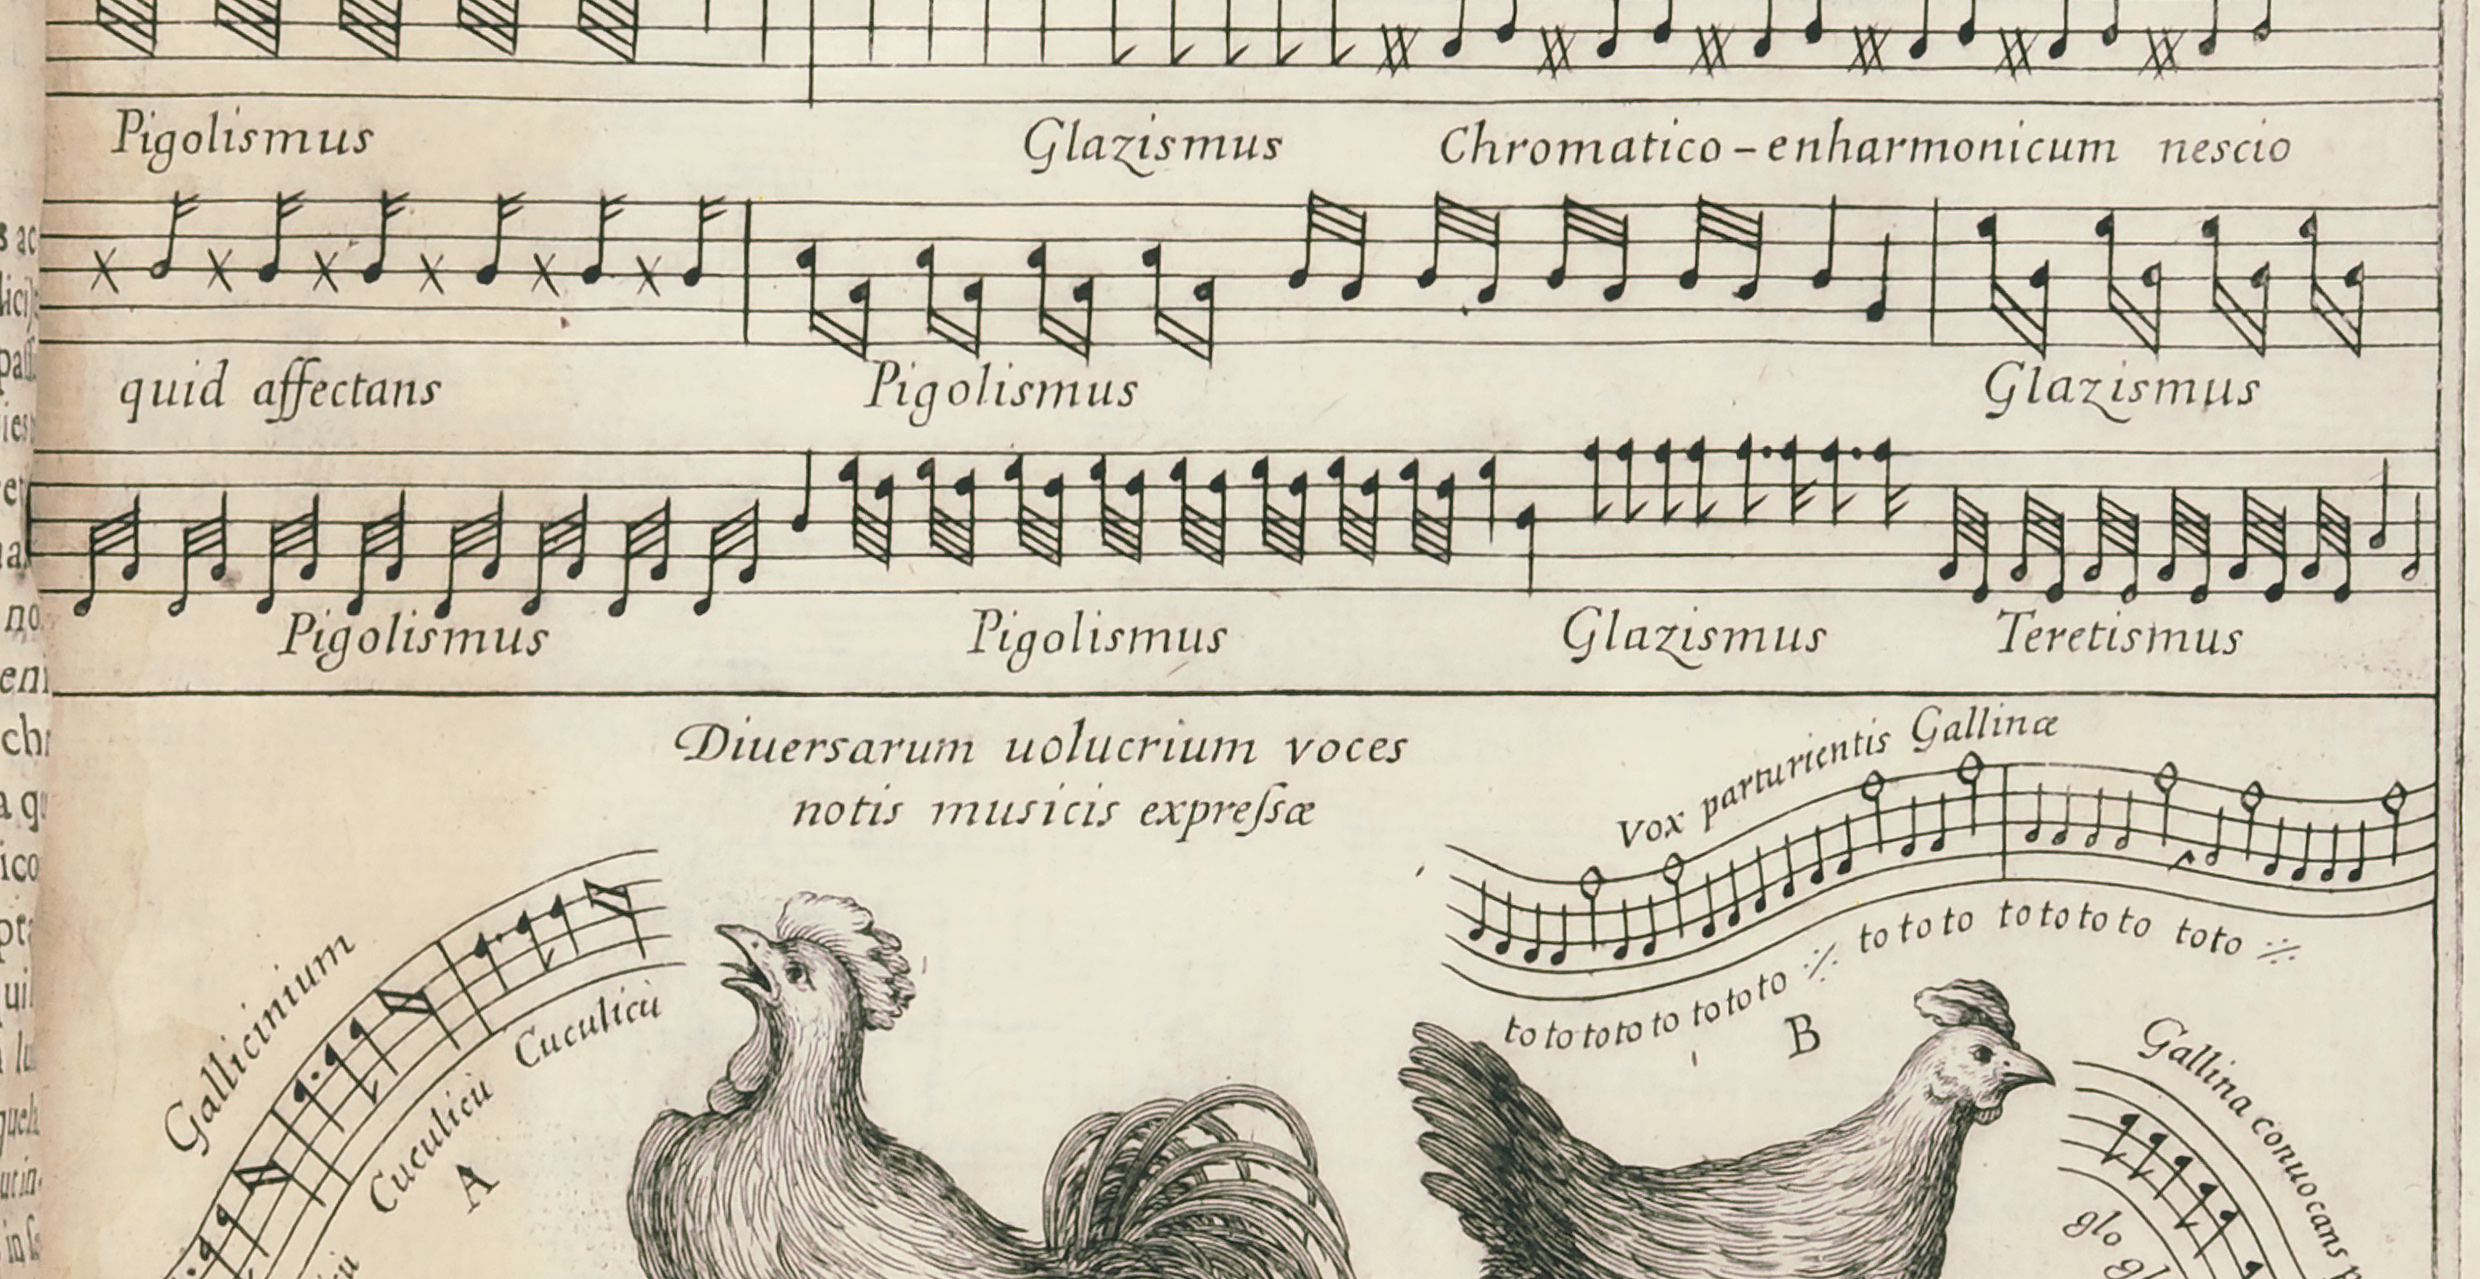
\includegraphics[width=\linewidth]{figures/chapter_1/musurgia.jpg}
    \mycaption{\textit{Musurgia Universalis, sive Ars Magna Consoni et Dissoni}}{
         'The Universal Musical Art, of the Great Art of Consonance and Dissonance', is a work by the Jesuit scholar Athanasius Kircher, published in 1650. Book one includes a rich discussion of bird song, including this illustration (Iconismus III), where the top part contains a study of \textit{Glottismi modulationum sibilo exprimendi in Luscinia observati}, or 'Modulations of the glottis to express whistling observed in Luscinia', which is contrasted with the much simpler vocalisations of cocks and hens. Reproduction in the public domain.
    }
    \label{c1_fig:musurgia}
\end{figure*}

While numerous examples of social learning and cultural phenomena exist in birds, it is their songs---thanks to their music-like qualities, and the remarkable ability of some species to imitate a wide range of sounds---that have garnered the most interest. Humanity's captivation with bird songs is also far from a recent development. As far back as 350 BCE., in his work 'Historia Animalium'. Aristotle noted that birds, especially 'broad-tongued' ones, were capable of learning their songs; and that, sometimes, their voices changed with the 'diversity of locality' (Book 4, Chapter 9). Aristotle's is one of the earliest recorded examples in a long tradition of analogies drawn between bird songs and human language and music across times and cultures \autocite{kleczkowska2015,zirin1980}.

Many centuries later, in 1650, the German Jesuit Athanasius Kircher would use musical notation to transcribe and analyse bird songs in his early musicology treatise, 'Musurgia Universalis', at a time when incorporating bird song-inspired phrases into instrumental compositions had become rather popular (See \autoref{c1_fig:musurgia}). However, it would not be until after the Industrial Revolution that technological advancements enabled the first recordings of singing birds, a crucial step in the study of changes and variations in their songs. (One earliest, if not the earliest, dates back to 1889 and was made by the pioneering sound recordist and broadcaster, Ludwig Koch, at the age of eight; \cite{britishlibrary2023}.) Fast-forward to the 1940s, and the invention of the sound spectrograph at the Bell Telephone Laboratories paved the way for a generation of researchers interested in bird song who were, for the first time, able to measure songs in unprecedented detail (\cite{baker2001a,koenig1946}; see \autoref{c1_fig:spectrograph}). An exhaustive study of the development of the song of the chaffinch \textit{Fringilla coelebs} by \textcite{thorpe1958} was followed by an explosion of interest in the matter, both in the field \autocite{Marler1962,marler1964} and the laboratory (see, for example, \cite{nottebohm1976} on the neurobiology of song production), which continues unabated to this day.

\begin{figure*}[bh!]
    \centering
    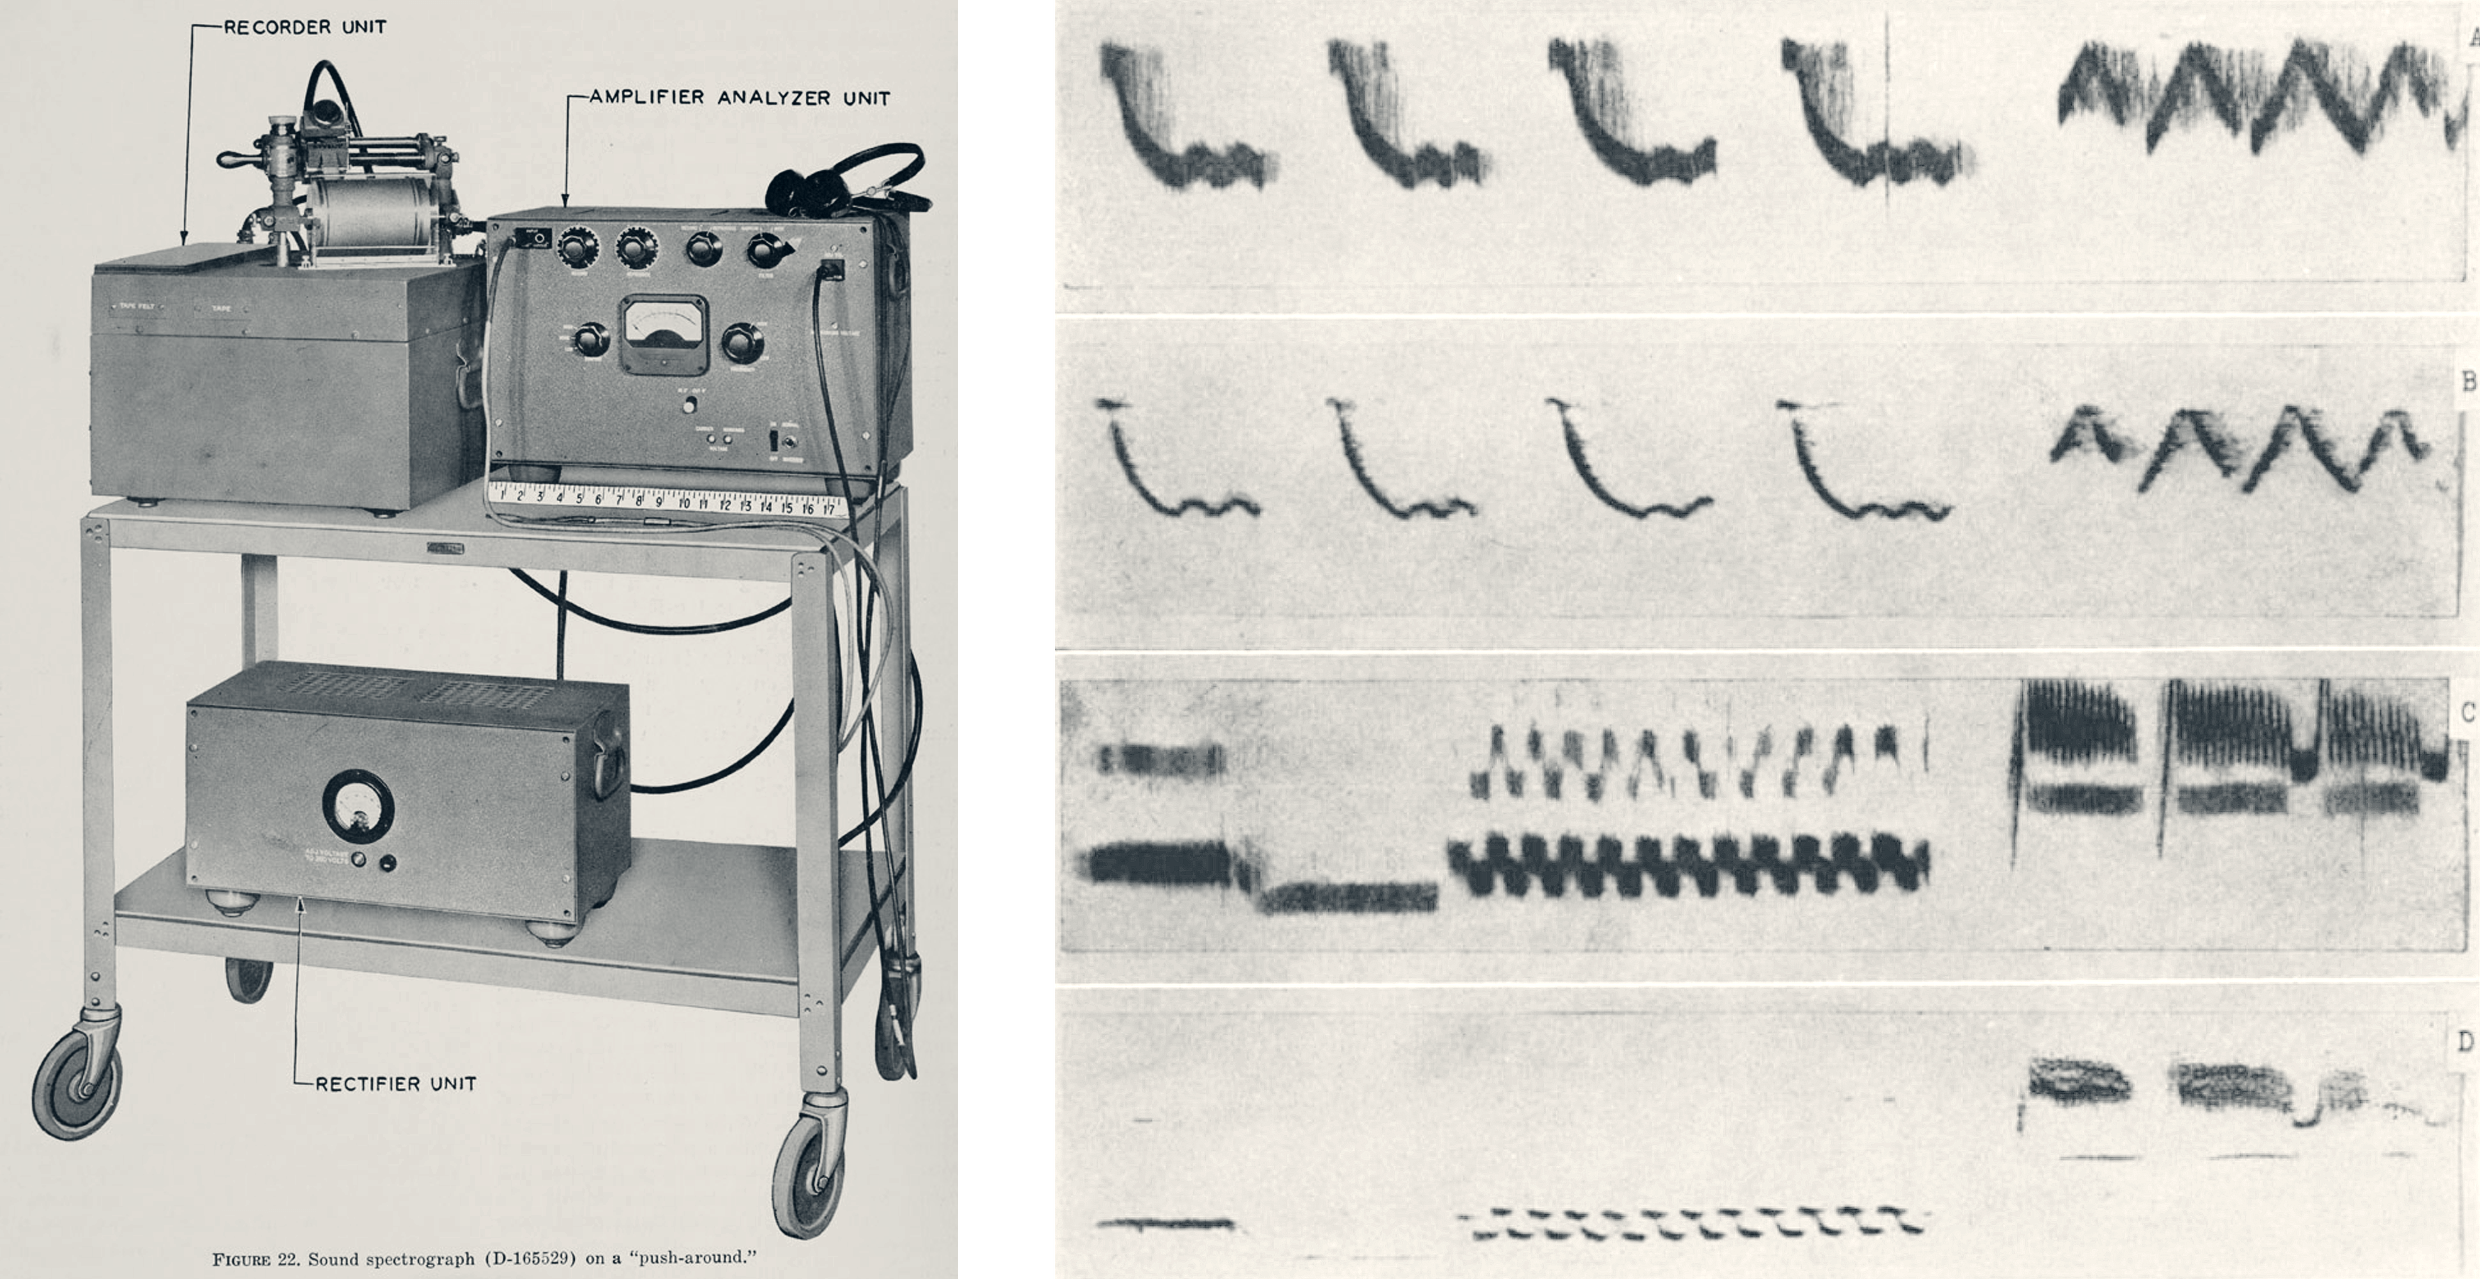
\includegraphics[width=\linewidth]{figures/chapter_1/spectrograph.png}
    \mycaption{Early spectrograph device and spectrograms of bird songs}{
        Left: Early magnetic tape spectrograph, built by Bell Telephone Laboratories circa 1946 around a modified commercial turntable.
        Right: Spectrograms of the songs of a nightingale \textit{Luscinia megarhynchos} (A, B) and a wood thrush \textit{Hylocichla mustelina} (C, D), generated from uncredited phonograph records. Both reproduced from \textcite{koenig1946}.
    }
    \label{c1_fig:spectrograph}
\end{figure*}


As researchers' fascination with animal cultures and the population consequences of song learning grew, they began describing cultural variation and longitudinal change in bird songs in great detail \parencite{nelson2017, zimmerman2016, zann1993, baptista1977, lachlan2003a}. This is well exemplified by the extensive research, over four decades, on a population of Savannah sparrows \textit{Passerculus sandwichensis} in Kent Island, New Brunswick, Canada \autocite{williams2013, mennill2018, williams2019, hensel2022, dixon1978}. Our growing understanding of bird song cultures, which forms the backdrop for this thesis, provides the most comprehensive evidence to date for the presence of culture and its evolution in non-human animals \autocite{slater2003a, aplin2019}. However, as with any behaviour, song learning is a complex process governed by numerous factors of diverse nature. To understand why change happens, we first need to understand why birds learn songs in the first place and the mechanisms behind change and variation.

\section{Why do some birds learn their songs?}
Most birds vocalise in one way or another, but the ability for vocal learning is a specialised trait found in only three orders: Psittaciformes, Apodiformes, and Passeriformes \autocite{kroodsma2004,packert2018}. Among passerines, commonly known as the perching birds, oscines (suborder Passeri) learn their songs, while suboscines (Tyranni) do not---although see \cite{searcy2021,tencate2021}. Song learning requires a significant investment of time, is metabolically costly, and requires a specialised syrinx and brain system, so the question arises: Why did it evolve, and why did it persist? Many hypotheses attempt to explain the potential advantages of vocal learning, which include a better ability to match the acoustic requirements of different habitats \autocite{hansen1979,rios-chelen2012}, the potential benefits of sharing songs with neighbours \autocite{payne1982}, and the ability of learned songs to serve as an 'honest signal' of developmental stability, nutritional status, and other indicators of fitness \autocite{Nowicki2002,ritchie2008}. Existing evidence suggests two primary functions: attracting and securing mates and deterring rivals \autocite{collins2004}. Nevertheless, there is considerable variation among species, and the current fitness consequences of song learning, on which these ideas are based, do not necessarily bear on its evolutionary origins.

Not all birds that learn their songs do so at the same point in their lives or for the same length of time. Some can only learn during the first months after they are born: Zebra finch \textit{Taeniopygia guttata} juveniles, for example, can only learn and develop their song roughly between 20 and 80 days after hatching \autocite{liu2004}. Other birds, such as the European starling \textit{Sturnus vulgaris},  can continue to learn, mimic, and perhaps invent new sounds throughout their lives. Furthermore, many birds that disperse early in their lives have a 'sensitive period' for learning that extends to the time when they establish their first territory \autocite{beecher2005,liu2004}. While this variation is often categorised as either 'open-ended' learning, where adults can keep learning, or 'closed-ended' learning, where songs solidify before the first year, it may be better viewed as a spectrum \autocite{brenowitz2005}. Lastly, there is remarkable variability in the size and complexity of the song repertoires among vocal learners. Some birds learn and endlessly sing a simple, single-syllable song, while others, like the brown thrasher \textit{Toxostoma rufum}, never seem to stop incorporating new sounds into their repertoires \autocite{Boughey1981}.

\section{(Some of) The forces that shape bird song}
Various factors shape the evolution of bird songs on a broad scale. These include physiological constraints on song production, the influence of past evolutionary trajectories (phylogenetic inertia), the acoustic environment, and sexual selection. Others, such as the dynamics of cultural transmission, learning biases, and the social, spatial, and demographic structure of populations, lead to changes in the relative frequencies of different song variations---that is, cultural evolution \autocite{whiten2019}. Although these processes and their often complex interactions all influence bird song, their relative importance is not well understood. We will briefly touch on some of them and then turn to those that have been least studied and are part of the focus of this thesis: demography's influence on cultural change and diversification in bird song, and structural biases that underpin cultural stability.

\subsection{Physiological constraints, phylogenetic inertia}
Birds produce their songs using an organ called the syrinx, which is located at the base of the trachea in an air sac close to the lungs \autocite{larsen2002a}. Its structure and precise location vary between species; those with more complex songs tend to have more syringeal muscles, which allows for precise control of sound \autocite{suthers2004}. The sounds produced by the syrinx are then filtered and modulated by the trachea and the beak, which together constitute the vocal tract \autocite{podos2004}. The body mass of a species is correlated with the size of its syrinx, which in turn influences the fundamental or lowest resonant frequency of the sounds that it can produce \autocite{martin2011,ryan1985a}. This means that vocal evolution will be constrained by any selective pressures impinging on body size, as well as the particular evolutionary trajectory of the species. The same is true for the morphology of the beak, which influences the pace at which a bird can produce notes and the range of their frequencies \autocite{derryberry2012,derryberry2018,podos2001,seddon2005}. These and other constraints, not least those derived from neural development and energy expenditure, determine the degrees of freedom available to other forces driving song evolution. 

\subsection{Ecological factors }
Sound propagates differently in different habitats. For example, vegetation attenuates sound amplitude, filters some frequencies more than others, and causes reverberation. Different physical environments have different levels of background noise; there may be sounds of abiotic origin, such as wind, streams, and rain, and a cacophony of other species striving to be heard. Songs, like any other signal, need to be detectable to be effective, and this process of acoustic adaptation is thought to be important in driving the evolution of song and other social signals (\cite{Endler1992,Grant2010,Tobias2010}; but see \cite{mikula2020}). On a shorter timescale, birds can respond to increased noise levels by adjusting the properties of their songs to reduce overlap with background noise, which they can do, for example, by increasing their minimum frequency \autocite{winandy2021, liu2020, derryberry2020, roca2016, nemeth2013, halfwerk2011, brumm2004}. However, it's not entirely clear whether this response is always driven by individual plastic responses or something that can also evolve across generations.

There are other ecological factors that can lead to song divergence: body size and beak morphology often change when a population of birds adapts to a different foraging niche, which, as mentioned earlier, can influence some of the acoustic and temporal features of songs as a byproduct \autocite{mayr1963,podos2001}. Additionally, songs can undergo changes when different bird species co-exist in the same habitat (sympatry). In such cases, selective processes may favour songs that can more easily distinguish birds from different species, which can help avoid the fitness costs of hybridization or aggressive interactions; a mechanism known as character displacement \autocite{seddon2005}. Interestingly, the opposite---convergent character displacement in sympatry---might also happen if better recognition of competitors is advantageous \autocite{grant1972, Tobias2014, Tobias2009}. 

\subsection{Sexual selection}
Bird song has traditionally been considered a male ornament that evolved through female preference. However, recent phylogenetic analyses suggest that, at least in oscine passerines, dimorphism in this trait is a consequence of multiple losses of elaborate female songs rather than gains in males \autocite{odom2014,odom2018}, and that the paucity of research on female song is significantly influenced by sociological factors \autocite{haines2020}. Indeed, most of the work done in the field of behavioural ecology over the past decades has focused on how females respond to songs and how males use them in territorial interactions. And, as a result, there is a vast literature detailing how songs can encode multiple messages and serve different, sexually selected functions, with great variation between species and sometimes inconsistent results (see \cite{catchpole2008} for reviews; also \cite{sierro2023} for recent work on this). To mention just a few themes: song frequency can be a reliable indicator of body size \autocite{ryan1985}, temporal and spectral consistency can evidence the nutritional stress suffered in early life \autocite{macdonald2006}, and sharing songs with other males can influence territory acquisition and the outcome of agonistic encounters \autocite{Demko2016a,krebs1978}.

\subsection{Learning biases and cultural dynamics}
For birds that learn their songs, the process itself introduces a host of new variables that can influence which songs a bird ultimately sings, their structure, and how they evolve over time. Initially, a bird needs to learn songs from another bird. Some birds may prefer specific 'tutors' over others, such as those that are older, louder, or sing more frequently \autocite{Greig2012}. This preference is variously referred to as a tutor, model, or demonstrator bias in the field of cultural evolution \autocite{kendal2015,VanDeWaal2010}. Cultural transmission of songs can occur in different ways. When songs are passed from parents to offspring, this is referred to as 'vertical transmission'. If songs are shared among birds in the same generation, it is known as 'horizontal transmission', and 'oblique transmission' when songs are learned from unrelated individuals in the previous generation \autocite{cavalli-sforza1982,ram2018}. Sometimes, tutor 'choice' can have extreme consequences: if a female pairs up with a male of a different species because he sings the same song as her father, and her father learnt the 'wrong' song, this can lead to the production of hybrid offspring \autocite{grant1997,grant1997a}.

Then, some songs may be preferred independently of who sings them---a 'content bias' \autocite{Richerson2005}. Song production is costly, and birds could favour learning easy-to-sing variants, or the opposite if singing difficult songs is rewarded with better reproductive resources. More broadly, however, there is a well-documented tendency for birds to preferentially learn the songs sung by members of their own species \autocite{slabbekoorn2002}, or even subspecies \autocite{nelson2000}. These preferences can arise through the interaction of innate biases for some regions of the syntactic or acoustic trait space, exposure to sounds during early life, and feedback loops during the learning process \autocite{feher2009,Feher2017,verzijden2012}. This interaction can be highly complex and shows great variability between species and even individuals \autocite{james2020,mets2017,mets2019,tencate2007}. 

Song acquisition in birds can also be influenced by how frequently they have heard a particular variant, or how many other birds sing it \autocite{aplin2015c,vanleeuwen2015}. The relationship between the frequency of a trait in a population and the probability that it is learned can be linear: if this is the case, transmission is unbiased. However, if more popular traits are more likely to be learned than would be expected given their frequency, learning is said to be conformist, or positively frequency-dependent. When the opposite is true the pattern is one of anti-conformism, or negative frequency dependence. Conformist learning seems to be a common strategy in nature, perhaps because it can help individuals leverage collective information to make decisions about locally adaptive behaviour \autocite{danchin2018,pike2010,whiten2019}; all else being equal, cultural traits will have a slower rate of change if their learning is conformist. Conversely, anti-conformist biases will cause faster turnover \autocite{acerbi2014} and might arise if individuals have a preference for novelty \autocite{Smaldino2015}.

Another determinant of the nature and pace of change in a population's songs is the precision with which birds learn them. Some authors have tried to calculate 'cultural mutation rates' for different species to reflect how much songs change from one generation to the next: Chaffinches, for example, appear to learn their songs very accurately \autocite{lachlan2003a,Slater1986}, which slows change. However, determining this quantity is complicated by the fact that many other factors also influence the pace of cultural change. One is the learning strategy used by individuals, as already mentioned. Another is the fact that songs can be modified during the learning process in non-random directions, in a process sometimes called convergent transformation or cultural attraction \autocite{claidiere2018,gray2007,heyes1993,morin2016}. This can be illustrated by an elegant experiment carried out by \textcite{feher2009}: song tutoring lineages were started with birds that were raised in isolation, and each new bird learned from the previous---mimicking natural generations of tutors and pupils. Many of the characteristic song features of the species emerged over the course of a few generations, presumably as a consequence of directional modifications introduced by the learners.

\subsubsection{Consequences of learning}
The available evidence suggests that the changes brought about by cultural dynamics are often neutral or even negative \autocite{langin2017,slater2003}, akin to random genetic drift \autocite{Grant2010}. However, in some cases, cultural change might help birds adapt to new acoustic landscapes \autocite{rios-chelen2012,slater2003}, or fine-tune the song's characteristics to better match the shifting perceptual preferences of the receivers \autocite{Renoult2019b}. At deeper timescales, the accumulation of neutral or directional cultural changes in songs might promote reproductive isolation between populations. However, although this possibility has attracted much interest, strong evidence for it is lacking \autocite{freeman2022,Lachlan2004,verzijden2012,Yeh2015}. More generally, and further complicating things, songs are not necessarily fixed behavioural packages, and different elements (notes, phrases, spectral properties, syntax) might change at different rates and be affected by different cultural, sexual, or ecological pressures (see, for example, \cite{williams2013}).

\subsection{Spatial, social, and demographic factors}
The most fundamental determinant of the interactions that lead to vocal learning in a population is the habitat that it occupies. Its physical features, vegetation structure, and distribution of resources, which are all tightly linked, bound the use of space made by individuals \autocite{spiegel2016, albery2021, firth2016}. This influences their social interactions and emergent social organisation (see \cite{he2019} for a review), which, in conjunction with dispersal and learning norms, ultimately dictates who learns from whom. For instance, spatial proximity will typically be correlated with vocal similarity if birds in a population learn their songs with some accuracy and their dispersal is limited---although the precise nature of this pattern depends on whether birds disperse before or after they learn, how many songs they learn, and from how many birds \autocite{ellers2003,williams1990}, as well as the many sources of learning bias discussed above. When birds remain close to the location where they learned, or if they selectively settle in places where they hear familiar songs, dialects or local song 'neighbourhoods' can emerge \autocite{podos2007}. It then follows that increased dispersal between any two areas within a population will promote vocal sharing and that the influx of immigrants from other populations can introduce new variation.

Space and movement play a significant role in how information flows and its impact on diversity. However, other factors, such as group size and turnover, also affect the speed of cultural change. First, smaller groups are more susceptible to stochastic factors, paralleling the effects of genetic drift on small populations \autocite{kimura1964}. As a consequence, smaller group sizes can increase the probability of extinction of any given song variant \autocite{nunn2009}, and lead to idiosyncratic changes in song structure \autocite{lachlan2013}. Second, higher background mortality and emigration will also lead to faster rates of change, independently of the learning strategy employed by individuals or the fidelity of their learning \autocite{nunn2009,Slater1986}.

Finally, a number of recent theoretical and experimental results suggest that the number, distribution, and connectedness of individuals in a population can influence the diversity and complexity of cultural traits in addition to their frequency distribution (see, for example, \cite{creanza2017,derex2018,derex2016,kempe2014}). While this phenomenon might be of great importance in human culture, bird songs are heavily constrained by ecological, cognitive, and sexual selective factors, which limits the potential of extrinsic factors to lead to appreciable gains in diversity or complexity. There is, however, some evidence from laboratory experiments that suggests that the availability of tutors and the quality of their instruction can reduce the influence of genetic contributions to the song phenotype \autocite{mets2017,mets2019}, and this mechanism could help explain the loss of song cultural diversity observed in some fragmented populations \autocite{hart2018,paxton2019}.

{\let\clearpage\relax\chapter*{\titlefont{This thesis}}}
\addcontentsline{toc}{chapter}{This thesis}

\section{Structure}
\lettrine[lines=2]Studying the processes that influence temporal and spatial patterns of bird song diversity in natural populations presents significant challenges. Although a long and fruitful history of field studies has provided us with examples of some of the processes outlined in the introduction, they often suffer from limitations such as small sample sizes, a lack of data for individual birds, and idiosyncratic analytical choices.

To address these challenges and contribute to the understanding of animal cultural diversity, as part of this thesis I introduce computational tools designed to efficiently collect and analyse extensive amounts of bird songs from the field (\autoref{chapter:2}). Then, I present and document the largest open-access dataset of songs from a single wild bird population to date, which includes comprehensive song and individual metadata, allowing researchers to rigorously test hypotheses that previously lacked robust support because of the limited data available for individual birds (\autoref{chapter:3}). It is perhaps worth noting that this field, like so many others, is increasingly reliant on technology and computational tools, which may pose a steep learning curve. In my case, transitioning from a background in fine arts and anthropology meant dedicating a substantial portion of my PhD to acquiring skills in statistics, high-performance computing, and programming---although I was also lucky to spend almost 9 months quite literally running around the woods!

\begin{figure*}[bh!]
    \centering
    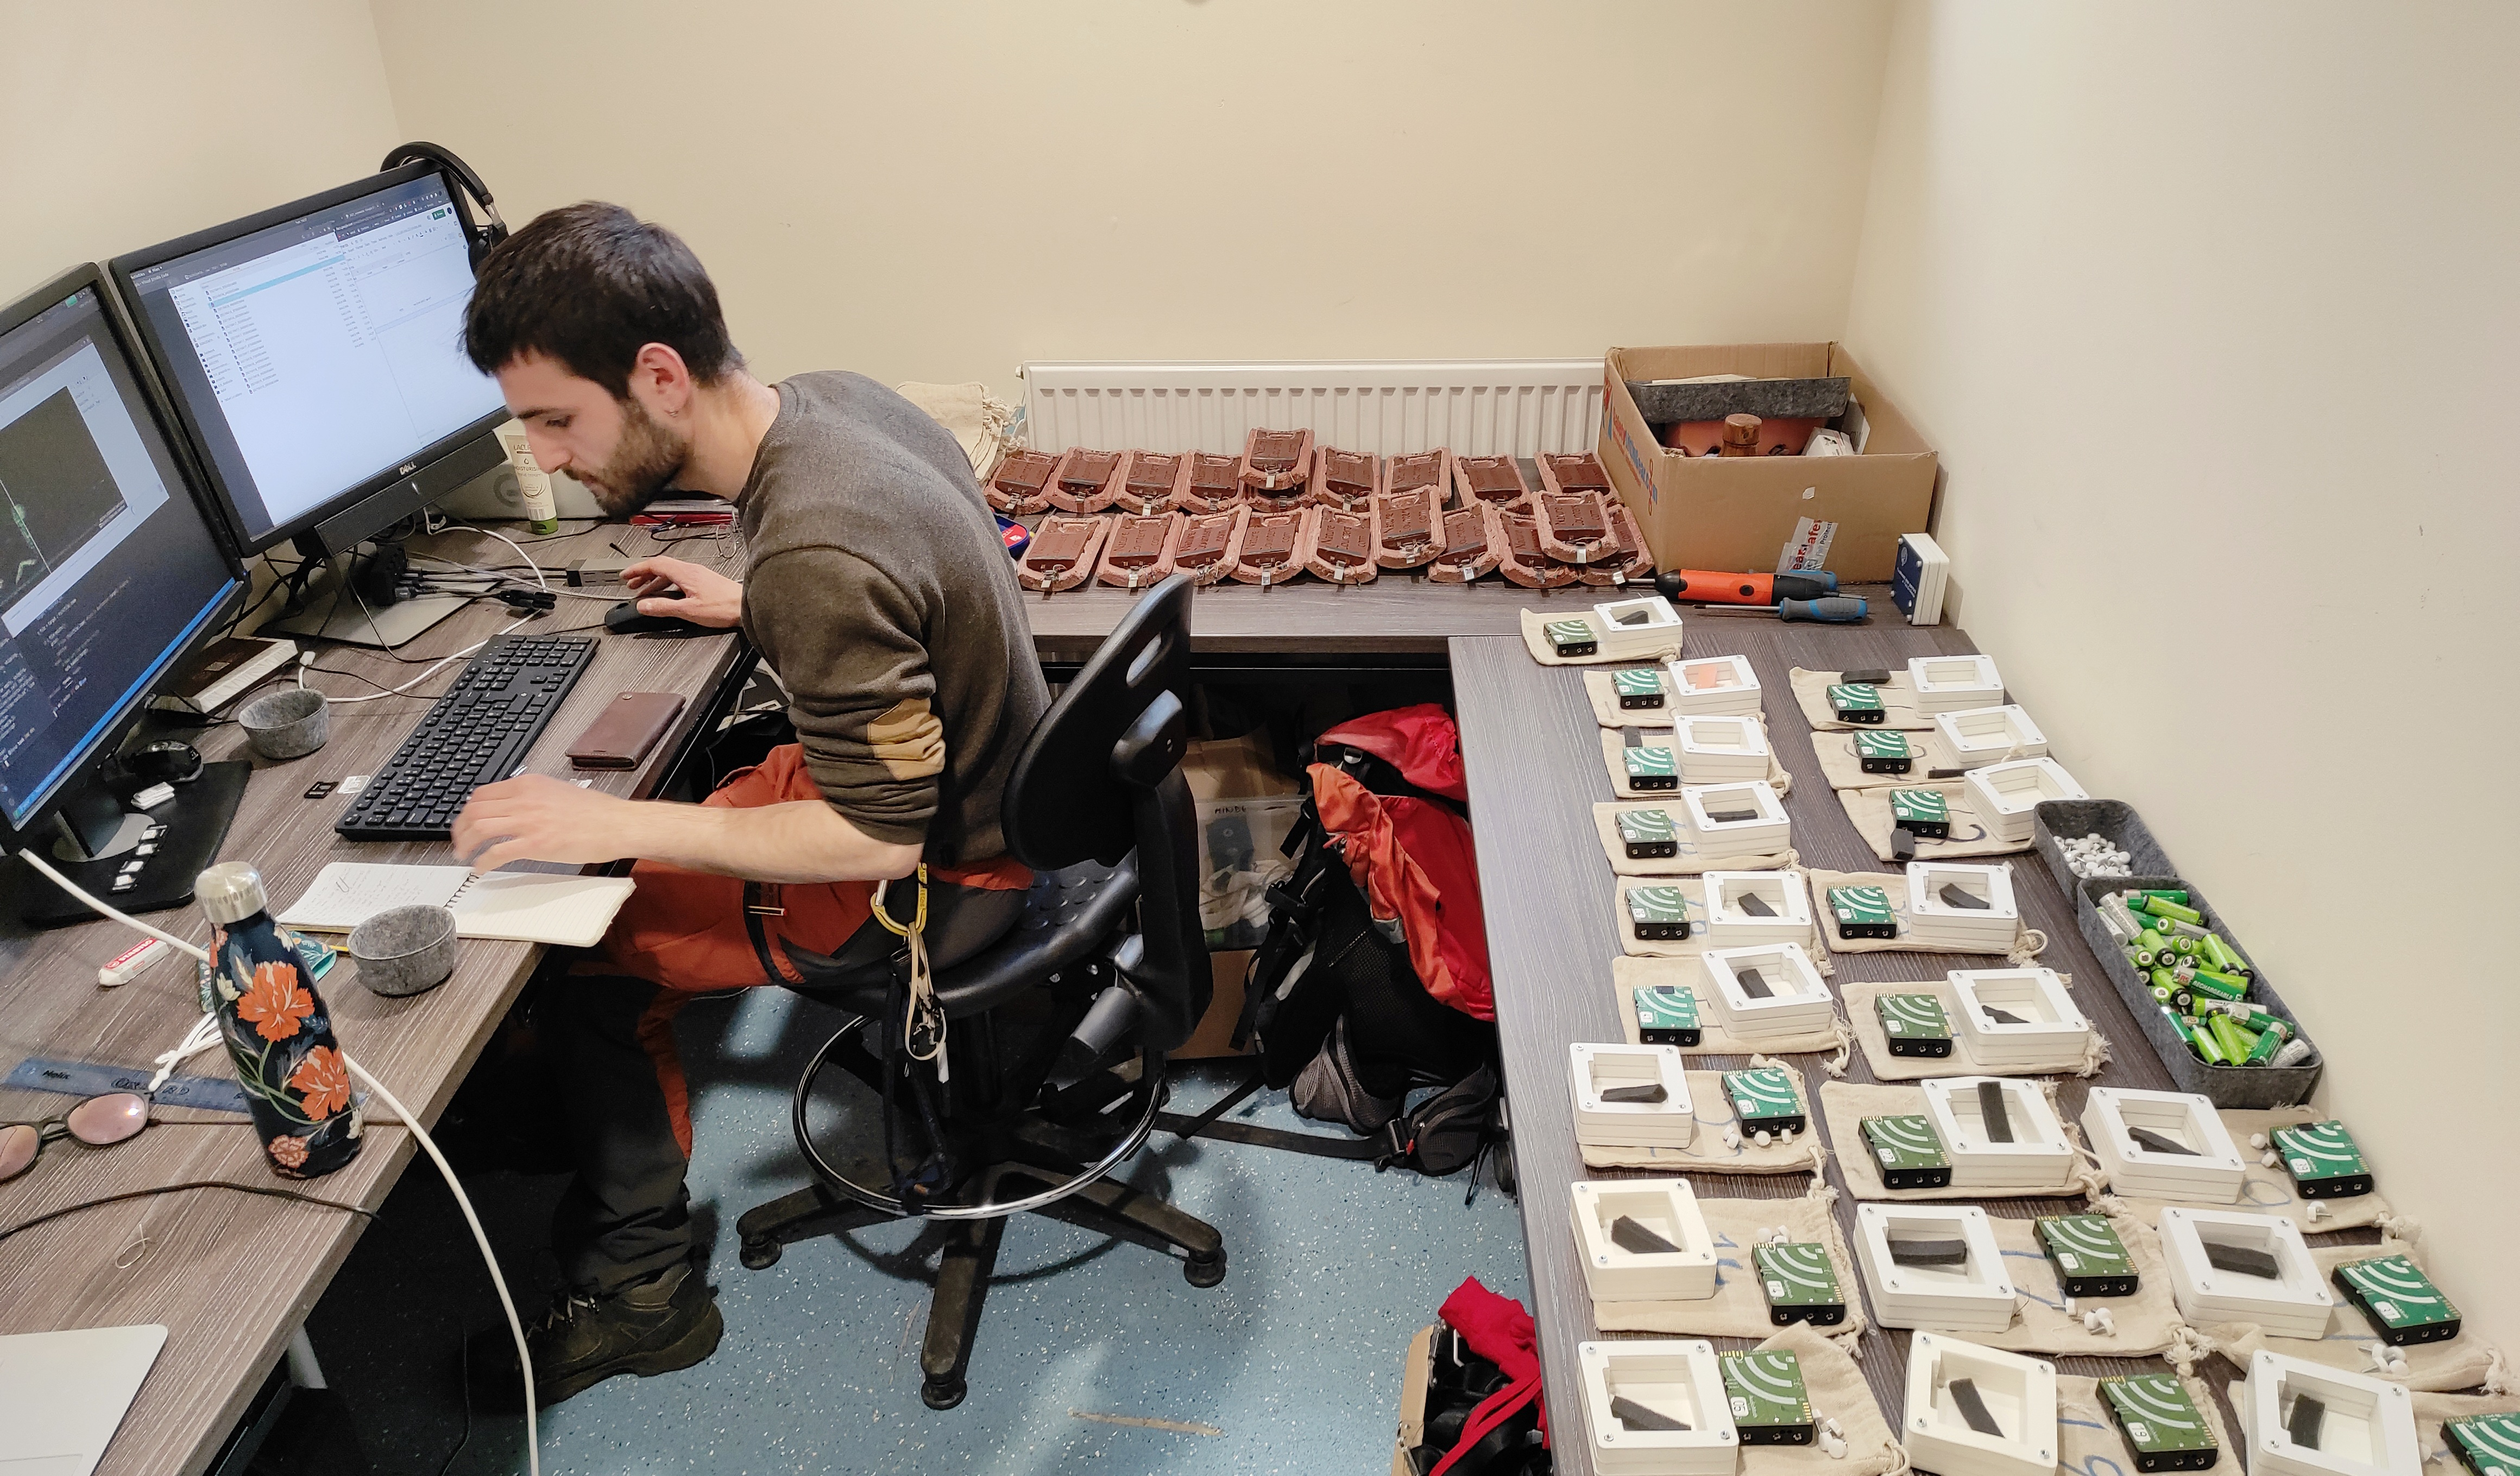
\includegraphics[width=\linewidth]{figures/chapter_1/nilo.jpg}
    \mycaption{The author (me!) in the field office, Wytham Woods, 2021}{
    }
    \label{c1_fig:nilo}
\end{figure*}

Having introduced the new software and data, which form the core of this thesis, I move on to its empirical section. As I briefly reviewed in the general introduction above, there has been extensive research on macroevolutionary patterns and social learning strategies or biases \parencite{pike2010, kendal2015, aplin2017, lachlan2018, tchernichovski2021}, but there remains a gap in our understanding of how demography contributes to the emergence and persistence of cultural traits in wild populations. Factors extrinsic to culture, like juvenile recruitment, emigration, mortality, and age structure, are thought to impact individuals' opportunities for learning and exposure to cultural variants \parencite{deffner2022a, deffner2022, kandler2023, fogarty2019, deffner2020, derex2016, kirby2021, nunn2009, barta2023}. But translating these expectations into empirical evidence remains a challenge; In this context, \autoref{chapter:4} of this thesis provides evidence that demographic factors are associated with cultural diversity and turnover at the individual and neighbourhood level, identifying the relevant spatial and temporal scale that drives emergent patterns within a wild bird population.

On the other hand, while we think that demographic factors can influence the pace of cultural change and promote or restrict diversity, they alone cannot explain why some song cultures are stably polymorphic, without collapsing into single variants or experiencing complete cultural replacement. It is generally assumed that innate mechanisms for accurate and conformist learning are the primary forces behind cultural stability in bird song \parencite{lachlan2018, lachlan2003a}. However, there is also growing support for the idea that perceptual, cognitive, and production biases, innate or culturally acquired, serve as attractors that can align the perception, memory, and reproduction of information among individuals and, as a consequence, enhance the fidelity of cultural transmission and limit the drift of cultural traits \parencite{feher2009, saldana2019, trehub2015}. In \autoref{chapter:5} I present some early evidence that the melodic space explored by a population of wild birds is highly non-random, in a way that parallels human musical traditions.

\begin{figure*}[th!]
    \centering
    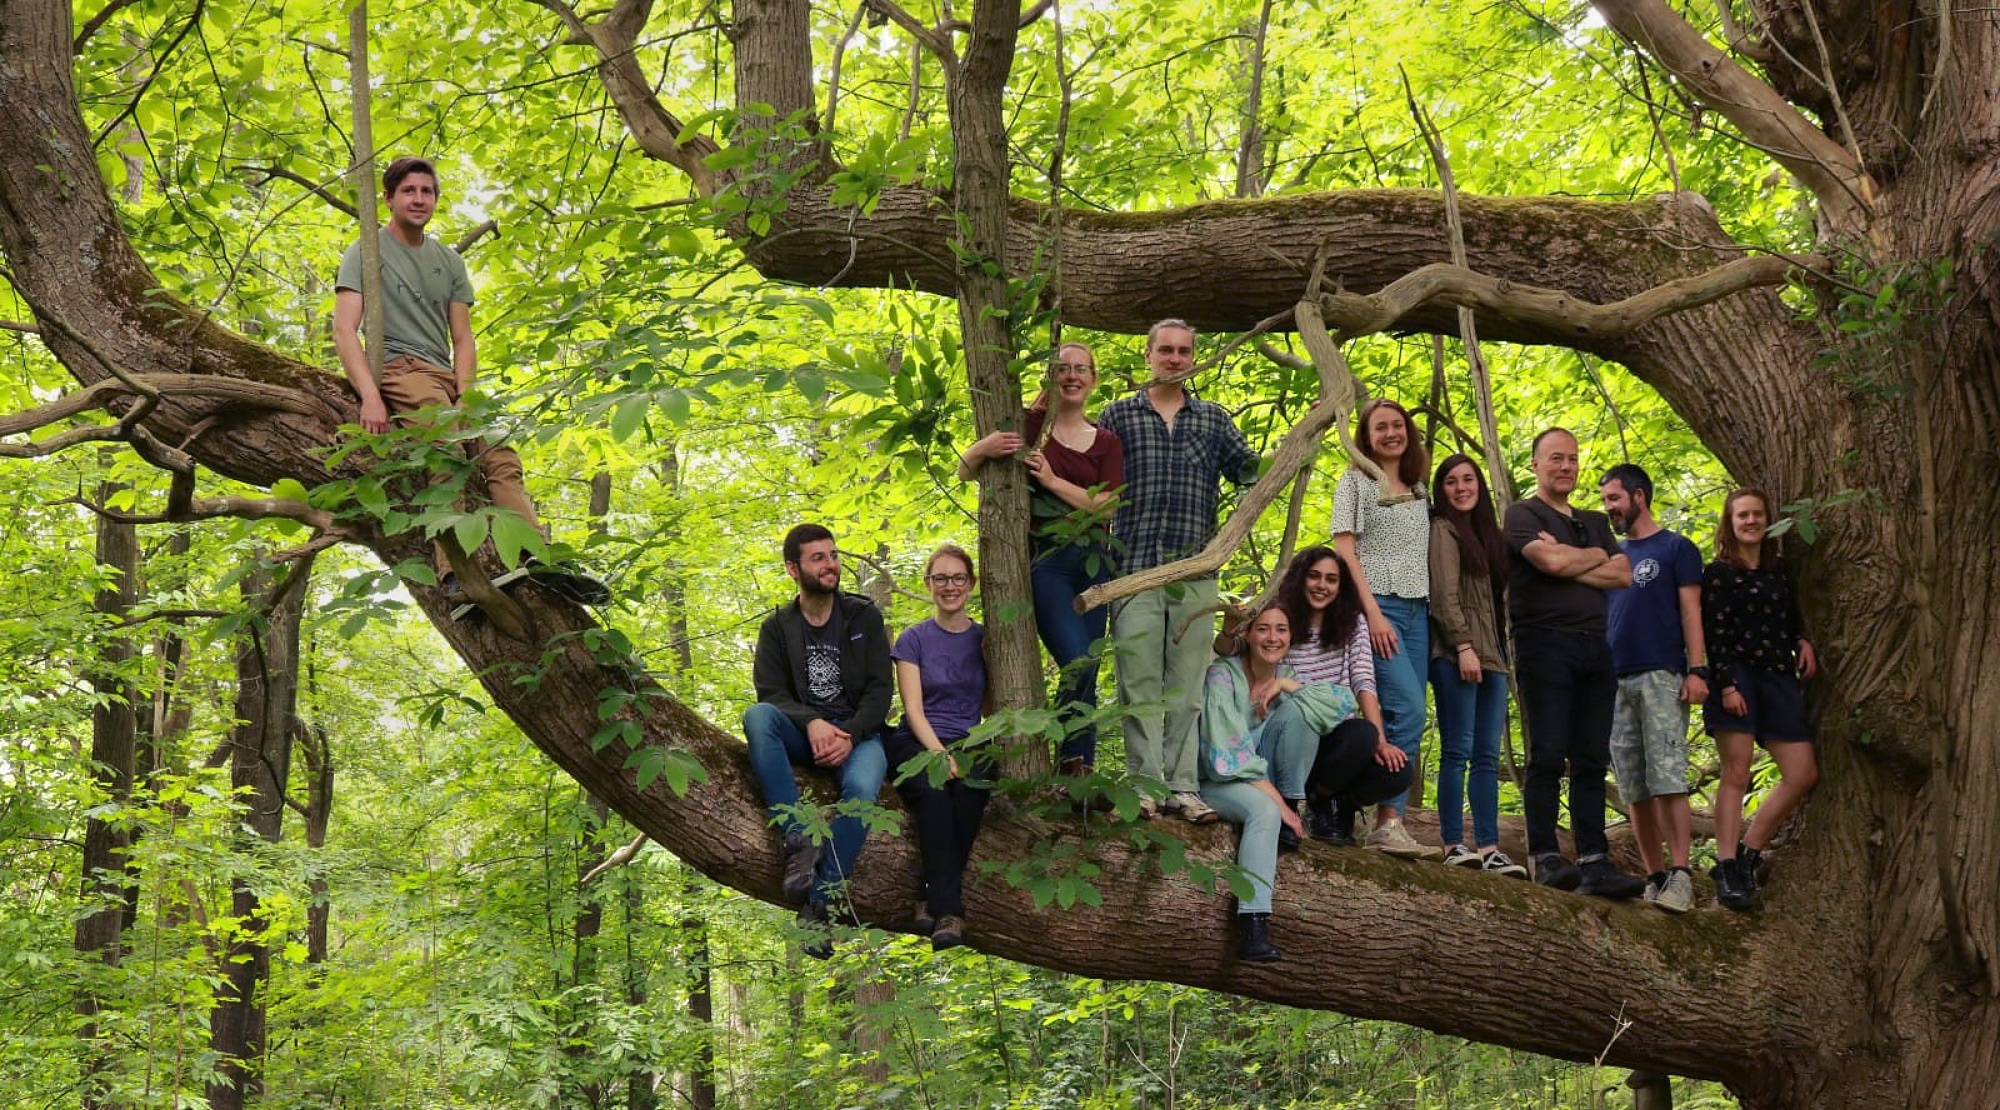
\includegraphics[width=\linewidth]{figures/chapter_1/wytham-group.jpg}
    \mycaption{Wytham Woods 2021 fieldwork season group photo}{
        From left to right:  Sam Crofts, Nilo Merino Recalde, Kristina Beck, Charlotte Regan, Joe Woodman, Anett Kiss, Carys Jones, Loanne Pichot, Andrea Estandía, Ben Sheldon, Keith McMahon, and Julia Haynes. 
    }
    \label{c1_fig:nilo}
\end{figure*}

\section{Study system}
I conducted all the research presented in this thesis within the long-term population study of great tits \textit{Parus major} in Wytham Woods, near Oxford, UK, which spans 76 uninterrupted years and has already recorded the life histories of nearly 120,000 individual birds \autocite{sheldon2022}. It began in 1947 with John Gibb and David Lack from the University of Oxford, initially with 100 nest boxes and later expanding to over 1000 around 1960. This study focuses primarily on great tits, a species that has become somewhat of a model species for various evolutionary, ecological, and cognitive studies in natural populations \autocite{aplin2017, Boyce1987, charmantier2008, cole2012,firth2018,Firth2016a,spurgin2019}. Their well-documented life history and behaviour, coupled with the characteristics of their songs, also make them ideal subjects for research on song learning and cultural change (see, for example, \cite{lambrechts1990, lind1996, rivera-gutierrez2010a, rivera-gutierrez2010, rivera-gutierrez2011, slagsvold1994, Ritschard2012}). 

Male great tits sing a repertoire of one to over ten simple song variants, each characterised by a small number of repeated notes that are repeated in a stereotypical manner \autocite{krebs1978,rivera-gutierrez2010a}. They primarily learn these songs from conspecifics during their first year, up to the point where they establish their own territory, and, consequently, are more likely to share their songs with neighbouring males than with other birds \autocite{mcgregor1982,mcgregor1989}. Research on great tit song conducted within the Wytham Woods population, in particular, has given rise to influential ideas and insights into bird singing behaviour, encompassing themes such as neighbour interactions, song matching, the connection between song repertoires and reproductive success \parencite{mcgregor1981, mcgregor1983, mcgregor1989}, dynamics of song learning \parencite{mcgregor1989, mcgregor1982b}, the role of song repertoires in maintaining territories \parencite{krebs1976, krebs1978}, the functions of dawn song \parencite{kacelnik1983, mace1987}, and the influence of spatial factors and movement on song culture \parencite{fayet2014}. 

I am not one to particularly cherish tradition in other aspects of life, but I feel honoured to be able to contribute---if much more modestly---to the rich history of research on bird song, and especially to do so here at Wytham. If you are about to read this thesis: thank you, and I hope it is not too painful.

\section{A few notes to the reader}
Each chapter in this thesis is a standalone piece of work. This means that some information, like the introduction to the study system and certain methods, is repeated in each chapter. To save time and avoid redundancy, \autoref{chapter:5}\S2 offers the most detailed description of the study system, fieldwork, and data annotation process.
Every chapter begins with a brief preface where I indicate the status of that specific manuscript and provide relevant resources. I have invested significant time into ensuring that all the code (over 25,000 lines, many more than in this thesis!) and the data generated during my PhD are easily accessible and reasonably well-documented, so that they may be useful to other students and researchers. You will find links to these resources within the manuscripts and highlighted in the respective prefaces.
I am told that hyperlinks will not work properly if, for some reason, you have printed this thesis on paper. Well, you shouldn't have, what can I say?

\renewcommand{\cleardoublepage}{}
\renewcommand{\clearpage}{}
\printbibliography

